% id: 35-29
% book: 쎈B 미적분1 · 03 미분계수와 도함수
% section: 유형 07 미분계수의 기하적 의미
% figure: tikz:fig-35-29
% answer: 
% answer_source: 
% variant_level: 0 (원본 전사)
% 이 파일은 build.mjs 가 items.json 에서 만든다. 고칠 때는 items.json 을 고친다.
\smash{\raisebox{1.5mm}{\dmkichul{쎈B 미적분1 35쪽 29번}}}
\noindent\begin{minipage}[t]{0.58\linewidth}\vspace{0pt}\raggedright 오른쪽 그림은 함수 $y=f(x)$의 그래프와 직선 $y=2x$를 나타낸 것이다. $0<a<b$일 때, 다음 중 옳지 \underline{않은} 것은?\end{minipage}\hfill\begin{minipage}[t]{0.4\linewidth}\vspace{0pt}\centering \resizebox{\ifdim\width>\linewidth\linewidth\else\width\fi}{!}{% 35-29(35쪽) — 원점을 지나며 위로 볼록하게 증가하는 y=f(x)의 그래프와 직선 y=2x, x축 위의 두 점 a, b(그래프까지 세로 점선).
% 스캔 화질이 낮아 TikZ 로 다시 그림. 눈금·좌표값은 원문에 없다.
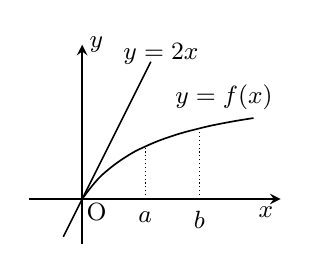
\begin{tikzpicture}[scale=0.8, line width=0.5pt]
  \draw[->, >=stealth, line width=0.7pt] (-0.85,0) -- (3.15,0) node[below left=-1pt, font=\small] {$x$};
  \draw[->, >=stealth, line width=0.7pt] (0,-0.72) -- (0,2.45) node[right=-1pt, font=\small] {$y$};
  \draw[line width=0.6pt] (-0.3,-0.6) -- (1.09,2.18);
  \draw[line width=0.6pt] plot[smooth, tension=0.75] coordinates {
    (0,0) (0.2,0.259) (0.4,0.455) (0.7,0.673) (1.0,0.833)
    (1.4,0.991) (1.86,1.121) (2.3,1.215) (2.72,1.285)};
  \draw[densely dotted, line width=0.4pt] (1.0,0) -- (1.0,0.833);
  \draw[densely dotted, line width=0.4pt] (1.86,0) -- (1.86,1.121);
  \node[below=1pt, font=\small] at (1.0,0) {$a$};
  \node[below=1pt, font=\small] at (1.86,0) {$b$};
  \node[below right=-2pt, font=\small] at (0,0) {$\mathrm{O}$};
  \node[font=\small] at (1.25,2.3) {$y=2x$};
  \node[font=\small] at (2.25,1.62) {$y=f(x)$};
\end{tikzpicture}
}\end{minipage}\par
\begin{choicesv}{$f(b)-f(a)<2(b-a)$}{$bf(a)-af(b)>0$}{$f'(a)>f'(b)$}{$f(a)<af'(a)$}{$f'(a+b)<f'(2\sqrt{ab}\mkern3mu )$}\end{choicesv}
